\documentclass[12pt, twoside]{article}
%\documentclass[12pt, twoside]{article}
\usepackage[letterpaper, margin=1in, headsep=0.2in]{geometry}
\setlength{\headheight}{0.6in}
%\usepackage[english]{babel}
\usepackage[utf8]{inputenc}
\usepackage{microtype}
\usepackage{amsmath}
\usepackage{amssymb}
%\usepackage{amsfonts}
\usepackage[nomessages]{fp} %\FPeval{\var-name}{2*sin(pi/6)}
\usepackage{siunitx} %units in math. eg 20\milli\meter
\usepackage{yhmath} % for arcs, overparenth command
\usepackage{tikz} %graphics
\usetikzlibrary{quotes, angles, arrows, arrows.meta}
\usepackage{pgfplots}
\usepgfplotslibrary{fillbetween}
\pgfplotsset{compat=1.16}
\usepackage{graphicx} %consider setting \graphicspath{{images/}}
\usepackage{parskip} %no paragraph indent
\usepackage{enumitem}
\usepackage{multicol}
\usepackage{venndiagram}

\usepackage{fancyhdr}
\pagestyle{fancy}
\fancyhf{}
\renewcommand{\headrulewidth}{0pt} % disable the underline of the header
\raggedbottom
\hfuzz=2mm %suppresses overfull box warnings

\usepackage{hyperref}

\fancyhead[LO]{La Scuola d'Italia / Dr.\ Huson / IB Math 11 \\* 19 October 2026}
\fancyhead[RO]{\fbox{\begin{minipage}{6cm}\footnotesize Nickname:\\[0.5cm]\end{minipage}}}
\fancyfoot[C]{\thepage}

\begin{document}
\subsubsection*{2 Homework: Slope, Lines and Systems of Equations}

\begin{enumerate}[itemsep=0.15cm]

%--- Problem 1: Gradient from two points; equation y = mx + c; axis intercepts; point on the line [9 marks] ---
%--- Source: Original (freshly authored, AA SL 2.1); Haese AA SL Ch. 1 ---
\item[1.]
The points $A(-2, 1)$ and $B(4, 4)$ lie on a straight line.

\begin{enumerate}[itemsep=0.1cm]
  \item Find the gradient (slope) of the line $AB$.
  \item Find the equation of the line $AB$ in the form $y = mx + c$.
  \item Find the $x$-intercept and the $y$-intercept of the line $AB$.
  \item The point $C(10, k)$ also lies on the line $AB$. Find the value of $k$.
\end{enumerate}

\begin{tikzpicture}
  \draw (-0.6,0) rectangle (14.6,5.4);
  \foreach \y in {1,2,...,5} \draw[dotted] (0,\y)--(14.1,\y);
\end{tikzpicture}

%--- Problem 2: General form 2x + 3y = 12; intercepts, gradient, perpendicular line, parallel line [9 marks] ---
%--- Source: Original (freshly authored, AA SL 2.1); Haese AA SL Ch. 1 ---
\item[2.]
The line $L_{1}$ has equation $2x + 3y = 12$.

\begin{enumerate}[itemsep=0.1cm]
  \item Find the $x$-intercept and the $y$-intercept of $L_{1}$.
  \item Find the gradient of $L_{1}$.
  \item The line $L_{2}$ is perpendicular to $L_{1}$ and passes through the
  point $(4, 1)$. Find the equation of $L_{2}$.
  \item The line $L_{3}$ is parallel to $L_{1}$ and has $y$-intercept $-2$.
  Write down the equation of $L_{3}$.
\end{enumerate}

\begin{tikzpicture}
  \draw (-0.6,0) rectangle (14.6,5.4);
  \foreach \y in {1,2,...,5} \draw[dotted] (0,\y)--(14.1,\y);
\end{tikzpicture}

\newpage

%--- Problem 3: Solve two 2x2 systems by hand (substitution, elimination) [6 marks] ---
%--- Source: Original (freshly authored, AA SL prior learning); Haese AA SL Ch. 1 ---
\item[3.]
Solve each system of equations. Show your working.

\begin{multicols}{2}
\begin{enumerate}[itemsep=0.1cm]
  \item $\begin{aligned}[t] 3x + 2y &= 16 \\ x - y &= 2 \end{aligned}$
  \item $\begin{aligned}[t] 2x + 3y &= 7 \\ 5x - 2y &= -11 \end{aligned}$
\end{enumerate}
\end{multicols}

\begin{tikzpicture}
  \draw (-0.6,0) rectangle (14.6,4.4);
  \foreach \y in {1,2,...,4} \draw[dotted] (0,\y)--(14.1,\y);
\end{tikzpicture}

%--- Problem 4: Read equation of a graphed line; graph x + y = 7; mark and state intersection; solve algebraically [9 marks] ---
%--- Source: Original (freshly authored, AA SL 2.1); Haese AA SL Ch. 1 ---
\item[4.]
The line $L$ is shown on the grid.

\begin{minipage}[t]{0.53\linewidth}
\vspace{0pt}
\begin{tikzpicture}[scale=0.6]
  \draw [thin, color=gray, xstep=1.0cm, ystep=1.0cm] (-2.5,-4.5) grid (8.5,8.5);
  % tick labels on the grid edges, clear of the lines
  \foreach \x in {-2,-1,0,1,2,3,4,5,6,7,8}
    \node[below] at (\x,-4.5) {$\x$};
  \foreach \y in {-4,-3,-2,-1,0,1,2,3,4,5,6,7,8}
    \node[left] at (-2.5,\y) {$\y$};
  \draw [thick, ->] (-2.5,0) -- (8.9,0) node [right] {$x$};
  \draw [thick, ->] (0,-4.5) -- (0,8.9) node [right] {$y$};
  % Line L: y = (3/2)x - 3
  \draw [very thick] (-1,-4.5) -- (7.667,8.5) node [right] {$L$};
\end{tikzpicture}
\end{minipage}
\hfill
\begin{minipage}[t]{0.45\linewidth}
\vspace{0pt}
\begin{enumerate}[itemsep=0.25cm]
  \item Write down the equation of $L$ in the form $y = mx + c$.
  \item The line $M$ has equation $x + y = 7$. Draw the line $M$ on
  the grid.
  \item Mark the point where $L$ and $M$ intersect on the grid. Write
  down its coordinates as an ordered pair.
  \item Use algebra to solve the system formed by the equations of $L$
  and $M$.
\end{enumerate}
\end{minipage}

\begin{tikzpicture}
  \draw (-0.6,0) rectangle (14.6,4.4);
  \foreach \y in {1,2,...,4} \draw[dotted] (0,\y)--(14.1,\y);
\end{tikzpicture}

\end{enumerate}
\end{document}
